
\documentclass[thmcnt=section, color=blue, 12pt]{my-elegantbook}

% Index page
\usepackage{imakeidx}
\makeindex[columns=2, intoc, options=-s index_style.ist]

% Title and author
\title{Mathematical Analysis}
\author{Isaac FEI}

% Reference file
\addbibresource{mathematical-analysis.bib} 

% Image of the book cover
\cover{cover}

\begin{document}

% Print title and cover page
\maketitle

%--------
% Preface
%--------

\frontmatter
\chapter*{Preface}

This book mainly follows the structure of \cite{apostolMathematicalAnalysisModern1974}.

%------------------------------

% Print table of contents
\tableofcontents
\mainmatter

%-------------------------------
% Main document starts from here
%-------------------------------

%==============================

\chapter{Point-Set Topology}

%==============================

\chapter{Functions of Bounded Variation and Rectifiable Curves}

%------------------------------ 

\section{Functions of Bounded Variation}

\begin{definition}
	Let $[a, b]$ be an interval.
	A set of points
	\begin{align*}
		P = \{ x_0, x_1, \dots, x_n \}
	\end{align*}
	satisfying
	\begin{align*}
		a = x_0 < x_1 < \cdots < x_n = b
	\end{align*}
	is called a \textbf{partition}\index{partition of an interval} of $[a, b]$.

	The interval $[x_{k-1}, x_k]$ is called the $k$-th subinterval of $P$,
	and we often write $\Delta x_k = x_k - x_{k-1}$.

	The collection of all partitions of $[a, b]$ is denoted by $\CALP [a, b]$.
\end{definition}


\begin{note}
	In mathematics texts, we have another definition of partitions,
	which states that a partition of a set $S$ is a collection of subsets of $S$
	such that they are disjoint and their union equals $S$.
	We should not confuse these two definitions.
\end{note}

\begin{definition}
	Let $f$ be a real-valued function on $[a, b]$.
	If $P = \{x_0, \dots x_n\}$ is a partition of $[a, b]$,
	write $\Delta f_k = f(x_k) - f(x_{k-1})$.
	If there exists a positive number $M$ such that
	\begin{align}
		\sum_{k=1}^n \abs{\Delta f_k} \leq M \label{eq:1}
	\end{align}
	for all partitions $P$ of $[a, b]$, then we say that $f$
	is \textbf{of bounded variation}\index{functions of bounded variation}
	on $[a, b]$.
\end{definition}

\begin{note}
	A geometric interpretation of the sum $\sum_{k=1}^n \abs{\Delta f_k}$
	is the total vertical length of several pieces of the function.
	Imagine a point moving along the curve of the function from the
	left to the right.
	If the partition gets finer and finer,
	then $\sum_{k=1}^n \abs{\Delta f_k}$
	will become the length of its journey projected on the $y$-axis.
	In fact, it is defined as the total variation as we shall introduce later.
\end{note}

Sometimes, it is convenient to denote the sum $\sum_{k=1}^n \abs{\Delta f_k}$
by the symbol
\begin{align*}
	v(P, f) := \sum_{k=1}^n \abs{\Delta f_k}
\end{align*}
We do not use the capital letter $V$ here for it is reserved for
the total variation.

A simple observation is that a function of bounded variation is also bounded.

\begin{proposition} \label{prop:2}
	Let $f$ be a function of bounded variation on $[a, b]$.
	Then $f$ is bounded on $[a, b]$.
\end{proposition}

\begin{proof}
	By definition, there exists $M > 0$ such that \eqref{eq:1} holds
	for any partitions of $[a, b]$.
	For any $x \in (a, b)$, consider the partition $P = \{a, x, b\}$.
	We have
	\begin{align*}
		\abs{f(x) - f(a)} + \abs{f(b) - f(x)} \leq M
	\end{align*}
	This implies that $\abs{f(x) - f(a)} \leq M$, which further
	implies $\abs{f(x)} \leq \abs{f(a)} + M$.
	Note that $x$ is arbitrarily chosen from $(a, b)$.
	Therefore, $f$ is indeed bounded on $[a, b]$.
\end{proof}

But a bounded function is not necessarily of bounded variation.

\begin{example} \label{eg:1}
	Consider the function
	\begin{align*}
		f(x) = \begin{cases}
			       \cos \frac{1}{x}, & x \in (0, 1] \\
			       0,                & x = 0
		       \end{cases}
	\end{align*}
	Its graph is shown in Figure~\ref{fig:1}.
	\begin{figure}[H]
		\centering
		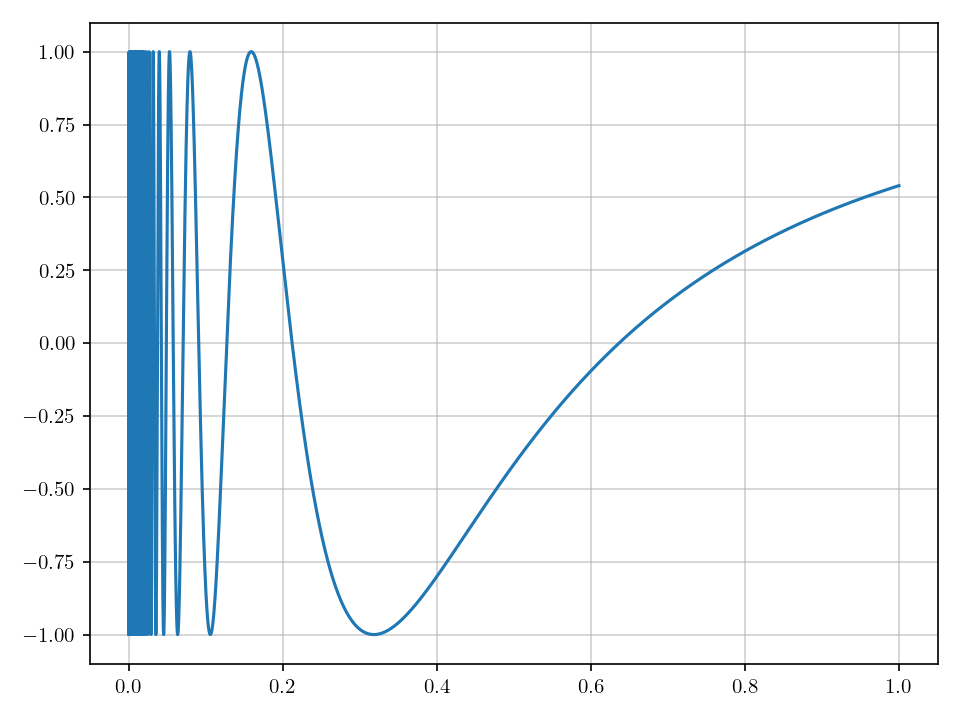
\includegraphics[width=0.6\textwidth]{figures/bounded-function-that-is-not-of-bounded-variation.png}
		\caption{Graph of the function $f(x) = \cos\frac{1}{x}$ for $x \in (0, 1]$ and $f(0) = 0$. It is bounded on $[0, 1]$ but not of bounded variation for it varies rapidly near $x=0$.}
		\label{fig:1}
	\end{figure}
	Clearly, this function is bounded by $1$.
	But intuitively, it is not of bounded variation since it varies rapidly
	near $x=0$.
	Let $P$ be a partition of $[0, 1]$ where each $x_k$ is given by
	\begin{align*}
		x_k = \begin{cases}
			      \frac{1}{(n-k) \pi}, & 1 \leq k \leq n-1 \\
			      0,                   & k = 0             \\
			      1,                   & k = n
		      \end{cases}
	\end{align*}
	For $k=1, \dots, n-1$, we have
	\begin{align*}
		f(x_k) = \cos ( (n-k) \pi ) \in \{-1, 1\}
	\end{align*}
	The function value is either $1$ or $-1$ and the sign alternates between
	each two consecutive points. Hence,
	\begin{align*}
		\sum_{k=1}^{n} \abs{\Delta f_k}
		\geq \sum_{k=2}^{n-1} \abs{\Delta f_k} = 2 (n - 2)
	\end{align*}
	As we increase the number of points in the partition, $\sum \abs{\Delta f_k}$
	will exceeds any given number.
	Therefore, $f$ is not of bounded variation on $[0, 1]$.
\end{example}

\begin{proposition} \label{prop:1}
	If $f$ is monotonic on $[a, b]$, then $f$ is of bounded variation on $[a, b]$.
\end{proposition}

\begin{proof}
	Assume $f$ is increasing.
	For any partition $P = \{x_0, \dots, x_n\}$ of $[a, b]$, we have
	\begin{align*}
		\sum_{k=1}^n \abs{\Delta f_k}
		= \sum_{k=1}^n (f(x_k) - f(x_{k-1}))
		= f(b) - f(a)
	\end{align*}
	Therefore, $f$ is of bounded variation on $[a, b]$.

	If $f$ is decreasing, then $-f$ is increasing.
	Applying what we have proved, we may conclude that $-f$ is of bounded variation.
	Hence, $f$ is also of bounded variation
	since $\sum \abs{\Delta (-f)_k} = \sum \abs{\Delta f_k}$.
\end{proof}

\begin{proposition} \label{prop:3}
	Suppose that $f$ is continuous on $[a, b]$ and the
	derivative $f^\prime$ exists in $(a, b)$.
	If $\abs{f^\prime(x)} \leq A$ for all $x \in (a, b)$,
	then $f$ is of bounded variation on $[a, b]$.
\end{proposition}

\begin{note}
	The assumption that $f$ being continuous on $[a, b]$,
	and $f^\prime$ exists in $(a, b)$ coincides with the mean value theorem.
	And indeed, it is the key of this proof.
\end{note}

\begin{proof}
	Let $P = \{x_0, \dots, x_n\}$ be a partition of $[a, b]$.
	By the mean value theorem, there exists $t_k \in (x_{k-1}, x_k)$
	for all $k=1, \dots, n$ such that
	\begin{align*}
		f(x_k) - f(x_{k-1}) = f^\prime(t_k) (x_k - x_{k-1})
	\end{align*}
	It then follows that
	\begin{align*}
		\sum_{k=1}^n \abs{\Delta f_k}
		 & = \sum_{k=1}^n \abs{f^\prime(t_k)} (x_k - x_{k-1}) \\
		 & \leq \sum_{k=1}^n A (x_k - x_{k-1})                \\
		 & = A (f(b) - f(a))
	\end{align*}
	Therefore, $f$ is of bounded variation on $[a, b]$.
\end{proof}

The following is a well crafted example of showing that
a continuous and differentiable function is not necessarily
of bounded variation
if we do not impose that its derivative is bounded in the interior.

\begin{example}
	Consider function defined on $[0, 1]$ given by
	\begin{align*}
		f(x) = \begin{cases}
			       x \cos \frac{\pi}{2x}, & x \in (0, 1] \\
			       0,                     & x = 0
		       \end{cases}
	\end{align*}
	Its graph is shown in Figure \ref{fig:2}.

	\begin{figure}[H]
		\centering
		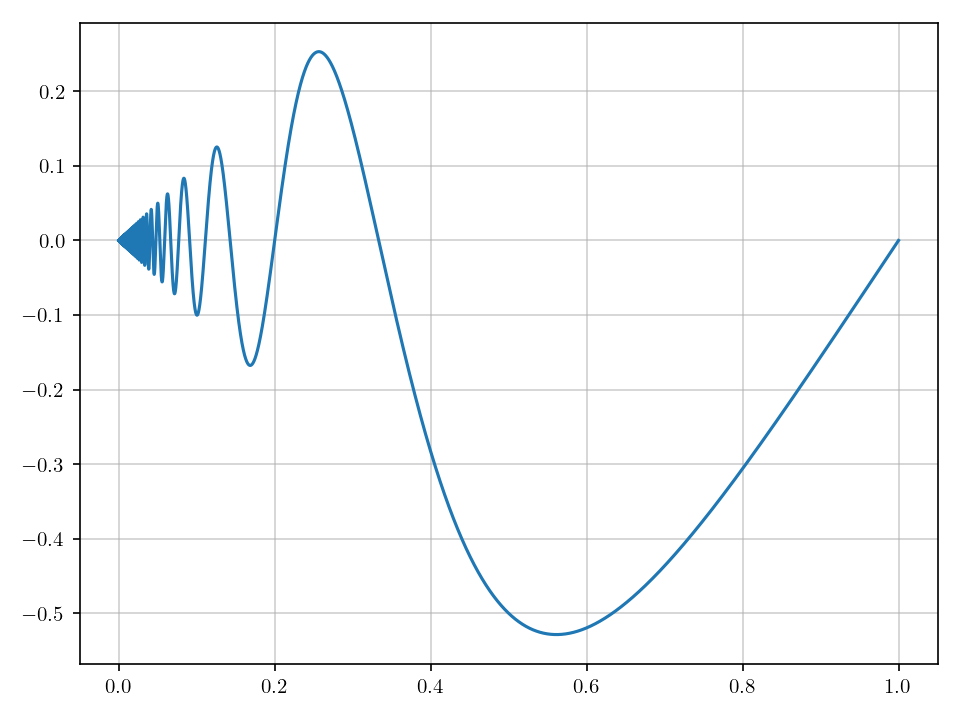
\includegraphics[width=0.6\textwidth]{figures/continuous-function-that-is-not-of-bounded-variation.png}
		\caption{Graph of the function $f(x) = x \cos \frac{\pi}{2x}$ for $x \in (0, 1]$ and $f(0) = 0$. This function is continuous and its derivative exists in $(0, 1)$. But the derivative is unbounded.}
		\label{fig:2}
	\end{figure}

	The fact that this function is not of bounded variation may be less intuitive
	than the one given in Example~\ref{eg:1}.
	The function still varies rapidly near $x=0$.
	However, it does not range from $-1$ and $1$.
	Instead, it damps out at $x=0$ and becomes $0$.
	But we will show in the following that we can find a partition so fine that
	by collecting each small function variation,
	the overall sum may still increase to infinity.

	Consider the partition
	\begin{align*}
		P = \{0, \frac{1}{2n}, \frac{1}{2n - 1}, \dots, \frac{1}{3}, \frac{1}{2}, 1\}
	\end{align*}
	We have
	\begin{align*}
		\sum_k \abs{\Delta f_k}
		 & = \frac{1}{2n} + \frac{1}{2n} + \frac{1}{2n - 1} + \frac{1}{2n - 1}
		+ \dots + \frac{1}{2} + \frac{1}{2}                                    \\
		 & = 1 + \cdots + \frac{1}{n}
	\end{align*}
	As $n$ gets larger and larger,
	the sum on the right hand-side will increase infinitely
	for we know that the harmonic series $\sum \frac{1}{n}$ diverges.
	Therefore, this function is not of bounded variation.
\end{example}

Of course, the condition of the derivative being bounded is not necessary
for a function to be of bounded variation.

\begin{example}
	The derivative of the square root function $f(x) = \sqrt{x}$ in $(0, 1)$
	is $f^\prime(x) = \frac{1}{2\sqrt{x}}$,
	which tends to infinity as $x \to 0$.
	But $f$ is clearly of bounded variation on $[0, 1]$
	by Proposition~\ref{prop:1} for it is increasing.
\end{example}

Let $P$ be a partition of $[a, b]$.
If we make it finer by adding some intermediate points,
then the sum of variations will increase.
This result may be helpful in some proofs.

\begin{proposition} \label{prop:4}
	Let $f$ be defined on $[a, b]$,
	and $P$ a partition of $[a, b]$.
	If $P^\prime$ is finer than $P$, i.e., $P^\prime \supset P$,
	then
	\begin{align*}
		v(P^\prime, f) \geq v(P, f)
	\end{align*}
\end{proposition}

\begin{note}
	Compare this to the upper and lower Darboux sums
	when we introduce them in a later section.
\end{note}

\begin{proof}
	It suffices to that prove for the case
	where $P^\prime$ is one point finer than $P$.
	Suppose $P = \{x_0, \dots, x_n\}$ and $P^\prime = P \sqcup \{c\}$.
	We have
	\begin{align*}
		v(P^\prime, f)
		 & = \abs{f(x_1) - f(x_0)} + \cdots
		+ \abs{f(c) - f(x_{j-1})} + \abs{f(x_j) - f(c)} + \cdots
		+ \abs{f(x_n) - f(x_{n-1})}            \\
		 & \geq \abs{f(x_1) - f(x_0)} + \cdots
		+ \abs{f(x_j) - f(x_{j-1})} + \cdots
		+ \abs{f(x_n) - f(x_{n-1})}            \\
		 & = v(P, f)
	\end{align*}
	\begin{note}
		Note that $j$ may equal to $1$ or $n$ in the above notations.
		We write down the summation in the expanded form
		to make the proof easier to read.
	\end{note}
	This completes the proof.
\end{proof}

%------------------------------ 

\section{Total Variation}

Recall that $f$ is said to be of bounded of variation
on $[a, b]$ if, equivalently to what we stated, the set
\begin{align}
	\set{\sum_{k=1}^n \abs{\Delta f_k}}{P \in \CALP [a, b]}
	\label{eq:2}
\end{align}
or with our shortened notation
\begin{align*}
	\set{v(P, f)}{P \in \CALP[a, b]}
\end{align*}
is bounded above.
This set is of course nonempty for $\{a, b\}$ is clearly a partition.
By the least upper bound property,
the set in \eqref{eq:2} has a supremum, which is referred to as
\textbf{total variation}\index{total variation} of $f$ on $[a, b]$.

\begin{definition}
	Let $f$ be of bounded variation on $[a, b]$.
	The total variation, denoted by $V_a^b (f)$,
	of $f$ on $[a, b]$ is defined as
	\begin{align*}
		V_a^b (f)
		:= \sup_{P \in \CALP [a, b]} v(P, f)
		= \sup \set{\sum_{k=1}^n \abs{\Delta f_k}}{P \in \CALP [a, b]}
	\end{align*}
\end{definition}

\begin{note}
	We adopt the notation $V_a^b(f)$,
	which is inspired by the notion of
	a definite integral $\int_a^b f(x) \dif x$.
	And as we shall see,
	these two concepts indeed share some similar properties, namely,
	the linear properties.

	Notations are very important for they provide intuitive expressions
	of the intrinsic mathematical concepts.
\end{note}

From this definition,
we have some simple observations.
First, the value of $V_a^b (f)$ is nonnegative.
And it is easy to prove that $V_a^b (f) = 0$
if and only if $f$ is constant on $[a, b]$.

The simplest function of bounded variation
(well, apart from a constant function) is
monotonic function.
It is natural to ask what is its total variation.
With a little thought,
one can imagine that
it should be the absolute value of the difference at the endpoints.

\begin{proposition}
	If $f$ is a monotonic function on $[a, b]$,
	then its total variation is the absolute value of the difference
	of the function values at the endpoints, i.e.,
	\begin{align*}
		V_a^b(f) = \abs{f(a) - f(b)}
	\end{align*}
\end{proposition}

\begin{proof}
	We only prove the case that $f$ is increasing.
	For any partition $P = \{x_0, \dots, x_n\}$ of $[a, b]$, we have
	\begin{align*}
		\sum_{k=1}^n \abs{f(x_k) - f(x_{k-1})}
		= \sum_{k=1}^n [f(x_k) - f(x_{k-1})]
		= f(b) - f(a)
	\end{align*}
	Note that the sum is independent of the partition.
	Hence, the set in \eqref{eq:2} is just a constant.
	Therefore, the total variation $V_a^b(f) = f(b) - f(a)$.
\end{proof}

When studying functions of bounded variation,
in most cases, we are often interested in
monotonic functions
or continuous and differentiable functions.
(Proposition~\ref{prop:1} and \ref{prop:3}.)

\begin{note}
	On one hand, we will see in Theorem~\ref{thm:4},
	a function is of bounded variation if and only if
	it can be expressed as a difference
	of two increasing functions,
	the need of studying monotonic functions arises naturally.

	On the other hand, as we shall see in the chapter on Riemann-Stieltjes integrals,
	we assume the integrator $\alpha$ is of bounded variation.
	Since integrator $\alpha$ will be put after the
	differential operator, $\dif \alpha$,
	and we often hope to express it as $\alpha^\prime(t) \dif t$
	to reduce the integral to Riemann integral
	and compute its value,
	we would like $\alpha$ to be differentiable.
\end{note}

But if we are curious about whether some piecewise functions
are of bounded variation,
then Proposition~\ref{prop:1} and \ref{prop:3} will not be enough.

\begin{example} \label{eg:2}
	For example, consider the following function defined on $[0, 3]$:
	\begin{align*}
		f(x) = \begin{cases}
			       x,           & 0 \leq x \leq 1 \\
			       -(x-1)(x-3), & 1 < x \leq 3
		       \end{cases}
	\end{align*}
	Figure~\ref{fig:4} depicts its graph.
	\begin{figure}[H]
		\centering
		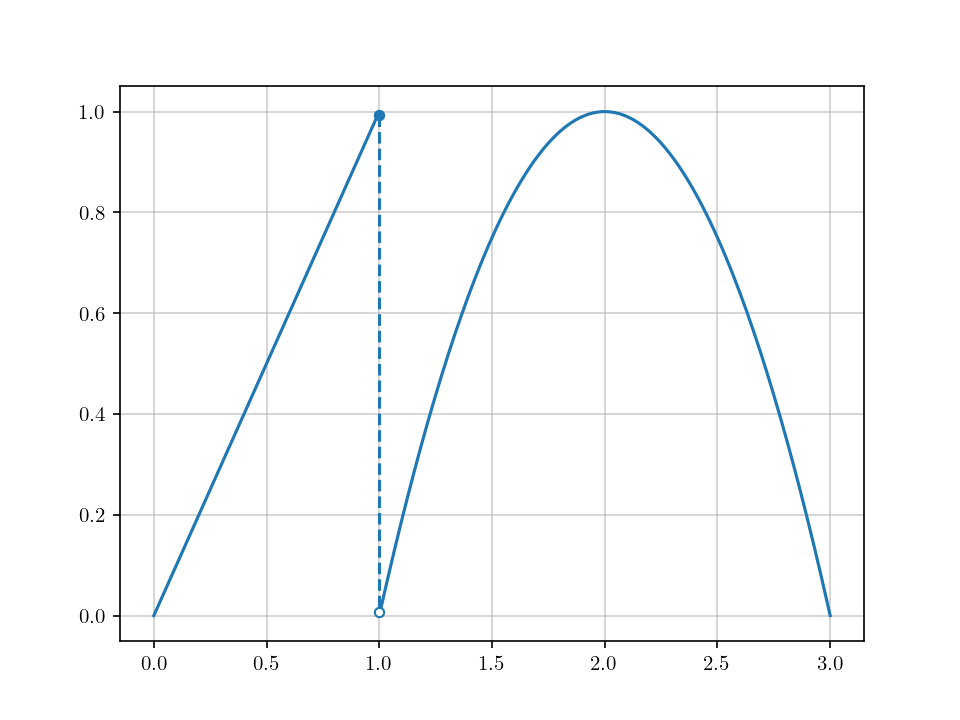
\includegraphics[width=0.6\textwidth]{figures/piecewise-function-of-bounded-variation.png}
		\caption{Is this function of bounded variation on $[0, 3]$?}
		\label{fig:4}
	\end{figure}

	Intuitively, the function in Figure~\ref{fig:4} should be of bounded variation.
	But we must be careful about the jump point,
	which we have not covered in the previous discussion.
\end{example}

\begin{proposition} \label{prop:5}
	Suppose $f$ is of bounded variation on $[a, b]$,
	and is continuous at $x = a$.
	If function $g$ is defined by revising the value at $x=a$, i.e.,
	\begin{align*}
		g(x) = \begin{cases}
			       f(x), & x \in (a, b] \\
			       y,    & x = a
		       \end{cases}
	\end{align*}
	then $g$ is still of bounded variation on $[a, b]$.
	And its total variation is given by
	\begin{align*}
		V_a^b(g) = V_a^b(f) + \abs{y - f(a)}
	\end{align*}
\end{proposition}

\begin{proof}
	Let $P$ be a partition of $[a, b]$.
	We have
	\begin{align}
		v(P, g) & = \abs{g(x_1) - g(a)} + \cdots \abs{g(x_n) - g(x_{n-1})}                                     \nonumber \\
		        & = \abs{f(x_1) - y} + \cdots \abs{f(x_n) - f(x_{n-1})}                                       \nonumber  \\
		        & \leq \left[ \abs{y -  f(a)} + \abs{f(x_1) - f(a)} \right] + \cdots \abs{f(x_n) - f(x_{n-1})} \nonumber \\
		        & = \abs{y - f(a)} + v(P, f)                                                                  \nonumber  \\
		        & \leq \abs{y - f(a)} + V_a^b(f)
		\label{eq:12}
	\end{align}
	This shows that $g$ is of bounded variation on $[a, b]$.

	Now, we compute its total variation.
	Let $\varepsilon > 0$ be arbitrary.
	Because $f$ is continuous at $x=a$,
	there exists $\delta > 0$ such that
	\begin{align*}
		\abs{x - a} < \delta \implies \abs{f(x) - f(a)} < \varepsilon/4
	\end{align*}
	By the definition of total variation and Proposition~\ref{prop:4},
	there exists a fine enough partition $P$
	such that the minimum length of the subinterval is less than $\delta$, and
	\begin{align*}
		v(P, f) > V_a^b(f) - \varepsilon/2
	\end{align*}
	On the subinterval $[a=x_0, x_1]$, we have
	\begin{align*}
		\abs{\Delta g_1} & = \abs{g(x_1) - g(x_0)}                                                                     \\
		                 & = \abs{f(x_1) - y}                                                                          \\
		                 & \geq \abs{f(a) - y} - \abs{f(x_1) - f(a)}                                                   \\
		                 & = \abs{f(a) - y} + \abs{f(x_1) - f(a)} -
		2\abs{f(x_1) - f(a)}                                                                                           \\
		                 & \text{Note that $\abs{x_1 - x_0} < \delta$, hence we may estimate the last term as follows} \\
		                 & > \abs{f(a) - y} + \abs{f(x_1) - f(a)} - 2 \cdot \varepsilon/4                              \\
		                 & > \abs{f(a) - y} + \abs{f(x_1) - f(a)} - \varepsilon/2
	\end{align*}
	\begin{note}
		When reaching
		\begin{align*}
			\abs{\Delta g_1} \geq \abs{f(a) - y} - \abs{f(x_1) - f(a)}
		\end{align*}
		in the above derivation,
		one may be worried that
		it is not proceeding towards the goal
		since we have a minus sign before $\abs{f(x_1) - f(a)}$.
		But since this term $\abs{f(x_1) - f(a)}$ can be made arbitrarily small,
		we can always add it (to construct the sum $v(P, f)$)
		and then subtract it,
		and make the trailing negative term $-2\abs{f(x_1) - f(a)}$ negligible,
		as what we did above.
	\end{note}
	It then follows that
	\begin{align*}
		v(P, g) > \abs{f(a) - y} + v(P, f) - \varepsilon/2
		> \abs{f(a) - y} + V_a^b(f) - \varepsilon
	\end{align*}
	Therefore, we have
	\begin{align*}
		V_a^b(g) \geq v(P, g) \geq \abs{f(a) - y} + V_a^b(f)
	\end{align*}
	Compare this to \eqref{eq:12}, we may conclude
	\begin{align*}
		V_a^b(g) = V_a^b(f) + \abs{f(a) - y}
	\end{align*}

\end{proof}

The function $f$ in Example~\ref{eg:2} can be regarded as a sum
of two functions on $[0, 3]$, $f(x) = g(x) + h(x)$ where
\begin{align*}
	g(x) & = \begin{cases}
		         x, & x \in [0, 1] \\
		         0, & x \in (1, 3]
	         \end{cases}            &  & = (x \mapsto x) \ind_{[0, 1]} \\
	h(x) & = \begin{cases}
		         0,            & x \in [0, 1) \\
		         \tilde{h}(x), & x \in [1, 3]
	         \end{cases} &  & = \tilde{h} \ind_{[1, 3]}
\end{align*}
where
\begin{align*}
	\tilde{h}(x) = \begin{cases}
		               -(x-1)(x-3), & x \in (1, 3] \\
		               0,           & x = 1
	               \end{cases}
\end{align*}

We have already seen that functions like $\tilde{h}$ are of bounded variation
in Proposition~\ref{prop:5}.
If we know the sum of two functions of bounded variation (on the same interval)
is also of bounded variation (Theorem~\ref{thm:1}),
we may then conclude that piecewise functions like $f$ in Example~\ref{eg:2}
are indeed of bounded variation.

Hence, the next step to do is studying
whether functions like $g$ and $h$ are of bounded variation.
Describing in words,
such functions are constructed
by extending a function of bounded variation
to a larger interval by defining function values of everywhere else
in the larger interval to be zeros.



\begin{theorem} \label{thm:1}
	Let $f$ and $g$ be of bounded variation on $[a, b]$, then
	so are their sum, difference and product.
	Moreover, we have the following inequalities:
	\begin{align}
		V_a^b (f \pm g)  \leq V_a^b (f) + V_a^b (g)
		\label{eq:3}
	\end{align}
	and
	\begin{align}
		V_a^b (fg)       \leq \sup_{x \in [a, b]} \abs{g(x)} V_a^b (f)
		+ \sup_{x \in [a, b]} \abs{f(x)} V_a^b (g)
		\label{eq:4}
	\end{align}
\end{theorem}

\begin{note}
	Note that the supremums in \eqref{eq:4} indeed exist
	since the functions $f$ and $g$ are bounded due to Proposition~\ref{prop:2}.
\end{note}

\begin{proof}
	We first show that the sum and the difference of two functions
	are of bounded variation, and satisfy \eqref{eq:3}.
	Let $P$ be an arbitrary partition of $[a, b]$.
	On each subinterval, we have
	\begin{align*}
		\abs{\Delta (f \pm g)_k}
		 & = \abs{f(x_{k}) \pm g(x_{k}) - [f(x_{k-1}) \pm g(x_{k-1})]} \\
		 & = \abs{\Delta f_k \pm \Delta g_k}                           \\
		 & \leq \abs{\Delta f_k} + \abs{\Delta g_k}
	\end{align*}
	Taking the sum over $k$, we have
	\begin{align*}
		\sum_{k} \abs{\Delta (f \pm g)_k}
		\leq \sum_{k} \abs{\Delta f_k} + \sum_k \abs{\Delta g_k}
		\leq V_a^b (f) + V_a^b (g)
	\end{align*}
	The above inequality shows that $f \pm g$ is of bounded variation on $[a, b]$,
	and \eqref{eq:3} is satisfied.

	In the following, we show that the product of two Functions
	are of bounded variation and satisfies \eqref{eq:4}.
	Let $P$ be an arbitrary partition of $[a, b]$.
	On each subinterval, we have
	\begin{align*}
		\abs{\Delta (fg)_k}
		 & = \abs{f(x_{k}) g(x_{k}) - f(x_{k-1}) g(x_{k-1})}                                \\
		 & \text{Add and subtract the term $f(x_{k-1})g(x_{k})$}                            \\
		 & = \abs{ g(x_{k})[ f(x_{k}) - f(x_{k-1})] + f(x_{k-1})[ g(x_{k}) - g(x_{k-1}) ] } \\
		 & \leq \abs{g(x_{k})} \abs{\Delta f_k} + \abs{f(x_{k-1})} \abs{ \Delta g_k }       \\
		 & \leq \sup_{x \in [a, b]} \abs{g(x)} \abs{\Delta f_k}
		+ \sup_{x \in [a, b]} \abs{f(x)} \abs{\Delta g_k}
	\end{align*}
	Summing over $k$, we have
	\begin{align*}
		\sum_k \abs{\Delta (fg)_k}
		\leq \sup_{x \in [a, b]} \abs{g(x)} \sum_k \abs{\Delta f_k}
		+ \sup_{x \in [a, b]} \abs{f(x)} \sum_k \abs{\Delta g_k} \\
		\leq  \sup_{x \in [a, b]} \abs{g(x)} V_a^b (f)
		+ \sup_{x \in [a, b]} \abs{f(x)} V_a^b (g)
	\end{align*}
	This shows the product $fg$ is in fact of bounded variation on $[a, b]$,
	and \eqref{eq:4} is satisfied.
\end{proof}

We must exclude the quotients from the above theorem
since the reciprocal $\frac{1}{f}$ of $f$ may not be of bounded variation
even though $f$ is.

\begin{example}
	Consider function
	\begin{align*}
		f(x) = \begin{cases}
			       1-x, & 0 \leq x < 1     \\
			       -x,  & 1 \leq x  \leq 2
		       \end{cases}
	\end{align*}
	Function $f$ is of bounded variation on $[0, 2]$ since it is decreasing.
	Its reciprocal is
	\begin{align*}
		\frac{1}{f(x)} = \begin{cases}
			                 \frac{1}{1-x}, & 0 \leq x < 1     \\
			                 -\frac{1}{x},  & 1 \leq x  \leq 2
		                 \end{cases}
	\end{align*}
	Figure \ref{fig:3} depicts the graphs of $f$ and $\frac{1}{f}$.
	\begin{figure}[H]
		\centering
		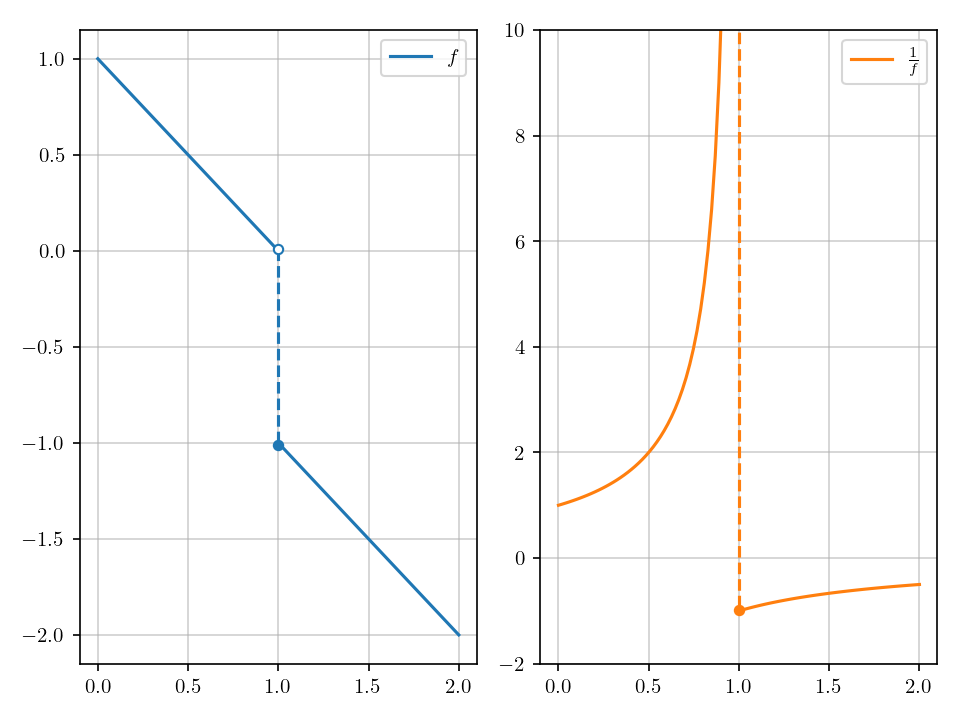
\includegraphics[width=0.6\textwidth]{figures/reciprocal-not-of-bounded-variation.png}
		\caption{Left: $f$ is of bounded variation for it is decreasing. Right: $\frac{1}{f}$ is not of bounded variation for it is unbounded.}
		\label{fig:3}
	\end{figure}
	Note that $\frac{1}{f}$ goes to positive infinity when $x \to 1^-$.
	Therefore, by Proposition~\ref{prop:2}, $\frac{1}{f}$ is not of bounded variation on $[0, 2]$
	since it is not bounded.
\end{example}

To extend Theorem~\ref{thm:1} to quotients,
we need to required that $f$ is bounded away from zero in the interval.

\begin{theorem}
	Let $f$ be of bounded variation on $[a, b]$.
	And there exists $m > 0$ such that $f(x) \geq m$ for all $x \in [a, b]$.
	Then the reciprocal of $f$ is of bounded variation on $[a, b]$, and
	\begin{align*}
		V_a^b ( \frac{1}{f} )
		\leq \frac{1}{m^2} V_a^b (f)
	\end{align*}
\end{theorem}

\begin{proof}
	Let $P$ be any partition of $[a, b]$.
	On each subinterval $[x_{k-1}, x_k]$, we have
	\begin{align*}
		\abs{\Delta (\frac{1}{f})_k}
		 & = \abs{\frac{1}{f(x_k)} - \frac{1}{f(x_{k-1})}} \\
		 & = \abs{\frac{\Delta f_k}{f(x_{k-1}) f(x_k)}}    \\
		 & \leq \frac{\abs{ \Delta f_k }}{m^2}
	\end{align*}
	Summing over $k$, we have
	\begin{align*}
		\sum_k \abs{\Delta (\frac{1}{f})_k}
		\leq \frac{1}{m^2} \sum_k \abs{\Delta f_k}
		\leq \frac{1}{m^2} V_a^b (f)
	\end{align*}
	Therefore, $\frac{1}{f}$ is of bounded variation on $[a, b]$.
\end{proof}

\subsection{Additive Property of Total Variation}

\begin{theorem} \label{thm:2}
	Let $f$ be of bounded variation on $[a, b]$, and $c \in (a, b)$.
	Then $f$ is of bounded variation on the subintervals $[c, b]$ and $[a, c]$.
	Moreover, we have
	\begin{align}
		V_a^b(f) = V_a^c(f) + V_c^b(f)
		\label{eq:9}
	\end{align}
\end{theorem}

\begin{proof}
	We will first show that $f$ is of bounded variation on each subinterval, and
	\begin{align}
		V_a^c(f) + V_c^b(f) \leq V_a^b(f)
		\label{eq:5}
	\end{align}

	Let $P^\prime$ and $P^{\prime\prime}$ be partitions of $[a, c]$ and $[c, b]$,
	respectively,
	and let $P = P^\prime \cup P^{\prime\prime}$.
	Note that $P$ is a partition of $[a, b]$,
	and by reviewing the notation of $v(P, f)$
	one may easily conclude that $v(P^\prime, f) + v(P^{\prime\prime}, f) = v(P, f)$.
	Since $f$ is of bounded of variation on $[a, b]$, we have
	\begin{align}
		v(P^\prime, f) + v(P^{\prime\prime}, f) = v(P, f) \leq V_a^b (f)
		\label{eq:6}
	\end{align}
	The above inequality holds for any partition $p^\prime$ of $[a, c]$
	and any partition $P^{\prime\prime}$ of $[c, b]$.
	Therefore, by definition, $f$ is of bounded variation on $[a, c]$ and $[c, b]$.
	Moreover, taking the supremum over $P^\prime$ and then over $P^{\prime\prime}$
	on both sides of \eqref{eq:6}, we will obtain exactly \eqref{eq:5}.

	To show the equality \eqref{eq:9}, we also need to show
	\begin{align}
		V_a^c(f) + V_c^b(f) \geq V_a^b (f)
		\label{eq:7}
	\end{align}
	Let $\varepsilon > 0$ be arbitrary.
	There exists a partition $P$ of $[a, b]$
	such that $v(P, f) > V_a^b(f) - \varepsilon$.
	Let
	\begin{align*}
		P^\prime = ( P \cap [a, c] ) \cup \{c\} \quad \text{and} \quad
		P^{\prime\prime} = ( P \cap [c, b] ) \cup \{c\}
	\end{align*}
	It is clear that $P^\prime$ and $P^{\prime\prime}$
	are partitions of $[a, c]$ and $[c, b]$, respectively.
	By Proposition~\ref{prop:4}, we have
	\begin{align}
		V_a^c(f) + V_c^b(f) \geq v(P^\prime, f)
		+ v(P^{\prime\prime}, f)
		\geq v(P, f) > V_a^b(f) - \varepsilon
		\label{eq:8}
	\end{align}
	Because \eqref{eq:8} holds for every $\varepsilon > 0$, \eqref{eq:7} is proved.
\end{proof}

Applying the above theorem, we can immediately conclude that $f$
is also of bounded variation on any interval contained in $[a, b]$.

\begin{corollary} \label{cor:1}
	If $f$ is of bounded variation on $[a, b]$,
	and $[c, d] \subseteq [a, b]$,
	then $f$ is also of bounded variation on $[c, d]$.
\end{corollary}

\begin{proof}
	With the given condition, we have $a \leq c < d \leq b$.
	If $c = a$ or $d = b$,
	then the assumption of this corollary reduces to the one in Theorem~\ref{thm:2}.

	Now, we assume that $a < c < d <b$.
	Regarding $c$ as an intermediate point in $[a, b]$,
	Theorem~\ref{thm:2} shows that $f$ is of bounded variation on $[c, b]$.
	Next, because $d \in (c, b)$, applying Theorem~\ref{thm:2} again,
	we conclude that $f$ is of bounded variation on $[c, d]$.
\end{proof}

\subsection{Total Variation as a Function of the Right Endpoint}

Suppose $f$ is of bounded variation on $[a, b]$.
For any $x \in (a, b)$.
Theorem~\ref{thm:2} tells us that $f$ is of bounded variation on $[a, x]$.
Therefore, we can regard $V_a^x (f)$ as a function of $x$.

\begin{note}
	This is very similar to considering $\int_a^x f(t) \dif t$ as a function
	of the upper limit of the integral, which
	again shows that our notation of the total variation rather helpful.
\end{note}

When $x = b$, it is just the total variation of $f$ on the entire interval.
We don't have definition for $x = a$ yet.
But we can easily fix this by naturally defining $V_a^a (f) := 0$.
Now, function $V_a^x(f)$ is defined on the entire interval $[a, b]$.

In the next chapter, we will study the Riemann-Stieltjes integral, which
is more generalized definition of the Riemann integral.
In the texts of the Riemann-Stieltjes integral $\int_a^b f \dif \alpha$,
we often assume that the integrator $\alpha$ is increasing
(or slightly more generalized, monotonic)\cite{rudinPrinciplesMathematicalAnalysis1976}.
But we can extend the results easily to a even more
general assumption that the integrator $\alpha$
is of bounded variation on $[a, b]$.

The key of achieving this is that a function of bounded variation
can be written as a difference of two increasing functions,
and conversely, the difference of two increasing functions
is of bounded variation
(Theorem~\ref{thm:4}).
And the following theorem tells us exactly how to
find such increasing
functions.

\begin{theorem} \label{thm:3}
	Let $f$ be of bounded variation on $[a, b]$.
	Then
	\begin{enumerate}
		\item $V_a^x(f)$ is increasing on $[a, b]$, and
		\item $V_a^x(f) - f(x)$ is also increasing.
	\end{enumerate}
\end{theorem}

\begin{proof}
	Let $h > 0$ (and $x + h \leq b$), by Theorem~\ref{thm:2}, we have
	\begin{align*}
		V_a^x (f) + V_x^{x+h} (f) = V_a^{x+h} (f)
	\end{align*}
	\begin{note}
		We have seen in Corollary~\ref{cor:1} that $V_x^{x+h}(f)$ indeed exists.
	\end{note}
	It then follows that
	\begin{align*}
		V_a^{x+h}(f) - V_a^{x}(f) = V_x^{x+h}(f) \geq 0
	\end{align*}
	This shows $V_a^x(f)$ is increasing.

	Next, we will prove $V_a^x(f) - f(x)$ is creasing.
	To ease the notation, let $g(x) = V_a^x(f) - f(x)$.
	Similarly, suppose $h > 0$ and $x + h \leq b$,
	consider the difference
	\begin{align}
		g(x+h) - g(x)
		= V_x^{x+h}(f) + [f(x+h) - f(x)]
		\label{eq:10}
	\end{align}
	\begin{note}
		Seeing the term $f(x+h) - f(x)$ in the context of total variation,
		we immediately think of the partition $P = \{x, x+h\}$ of $[x, x+h]$.
	\end{note}
	We have
	\begin{align*}
		\abs{f(x+h) - f(x)} \leq V_x^{x+h}(f)
	\end{align*}
	It then follows that
	\begin{align*}
		V_x^{x+h}(f) \geq \abs{f(x+h) - f(x)} \geq -[f(x+h) - f(x)]
	\end{align*}
	which further implies
	\begin{align}
		V_x^{x+h}(f) + [f(x+h) - f(x)] \geq 0
		\label{eq:11}
	\end{align}
	Comparing \eqref{eq:10} and \eqref{eq:11}, we conclude
	that $g(x)$ is indeed increasing.
\end{proof}

\subsection{Characterization of Functions of Bounded Variation}

With the help of Theorem~\ref{thm:3}, we can easily prove
the following elegant theorem,
which characterizes functions of bounded variation.
It states that a function on $[a, b]$ is of bounded variation
if and only if it can be written as a difference of two increasing functions.
The difficult part of find such increasing functions
is already handled by Theorem~\ref{thm:3}.

\begin{theorem} \label{thm:4}
	Let $f$ be defined on $[a, b]$,
	then $f$ is of bounded variation if and only if
	it can be expressed as a difference of two
	increasing functions.
\end{theorem}

\begin{proof}
	We first suppose that $f$ is of bounded variation.
	Then Theorem~\ref{thm:3} shows that $V_a^x(f)$
	and $V_a^x(f) - f(x)$ are both increasing on $[a, b]$.
	Since we can write
	\begin{align*}
		f(x) = V_a^x(f) - [ V_a^x (f) - f(x)]
	\end{align*}
	It is proved.

	Reversely, suppose that $f$ can be expressed as a difference of
	two increasing functions $g$ and $h$ on $[a, b]$, $f = g - h$.
	Proposition~\ref{prop:1} tells us that $g$ and $h$ are of bounded variation
	since they are increasing functions.
	Then by Theorem~\ref{thm:1}, we know that $g - h$ is also of bounded variation.
	This completes the proof.
\end{proof}

\begin{note}
	We can also make these two increasing functions strict.
	Suppose $f = g - h$.
	We can easily achieve this by defining $\tilde{g}(x) = g(x) + x$
	and $\tilde{h}(x) = h(x) + x$.
\end{note}

\section{Continuous Functions of Bounded Variation}

Previously, we have shown that a function $f$ of bounded variation can be
written as the difference of two increasing functions, $f = g - h$.
Now, suppose $f$ is continuous.
We will show in this section that the two increasing functions $g$ and $h$
can also be made continuous as well.

\begin{theorem}
	Suppose $f$ is of bounded variation on $[a, b]$.
	Then $f$ is continuous at $x_0 \in [a, b]$
	if and only if $V_a^x(f)$ is continuous at $x_0$.
	In other words, every point of continuity of $f$ is also
	a point of continuity of $V_a^x(f)$ and vice versa.
\end{theorem}

\begin{proof}
	We first suppose that $V_a^x(f)$ is continuous at $x_0$
	and show that $f$ is also continuous at $x_0$,
	which is the easier direction to prove.

	We will only show that $f$ is continuous from the right at $x_0$ ($x_0 \neq b$),
	and the continuity from the left is similarly proved (including $x_0 = b$).
	Let $\varepsilon > 0$ be arbitrary.
	Because $V_a^x(f)$ is continuous at $x_0$,
	there exists $\delta  > 0$ such that
	\begin{align*}
		\abs{x - x_0} < \delta \implies \abs{V_a^x(f) - V_a^x(f)} < \varepsilon
	\end{align*}
	For all $h$ satisfying $0 < h < \delta$, we have
	\begin{align*}
		\abs{f(x_0 + h) - f(x_0)}
		 & = v(P, f) \quad \text{where $P = \{x_0, x_0+h\}$ is a partition of $[x_0, x_0+h]$} \\
		 & \leq V_{x_0}^{x_0+h}(f)                                                            \\
		 & = V_a^{x_0+h}(f) - V_a^{x_0}(f)                                                    \\
		 & < \varepsilon
	\end{align*}
	This shows that $f$ is continuous at $x_0$ from the right.
	Applying a similar argument,
	one may show that it is also continuous at $x_0$ from the left
	by considering the interval $[x_0-h, x_0]$.

	We now prove the reverse direction.
	Suppose $f$ is continuous at $x_0$.
	Again, we will only prove that $V_a^x(f)$
	is continuous at $x_0$ ($x_0 \neq b$) from the right.
	Let $\varepsilon > 0$ be arbitrary.
	Since $f$ is continuous at $x_0$, there exists $\delta > 0$
	such that
	\begin{align*}
		\abs{x-x_0} < \delta \implies \abs{f(x) - f(x_0)} < \varepsilon/2
	\end{align*}
	Consider the total variation $V_{x_0}^b(f)$.
	For any $h$ satisfying $0 < h < \delta$,
	There exists a partition $P$ such that
	\begin{align*}
		x_1 - x_0 \leq \delta
	\end{align*}
	where $x_1 = x_0 + h$
	and
	\begin{align}
		v(P, f) > V_{x_0}^b(f) - \varepsilon/2
		\label{eq:14}
	\end{align}
	\begin{note}
		If one is confusing about how finding such $P$ is possible,
		we can think of finding it with the following process.
		First, find a partition $P$ of $[x_0, b]$ such that
		\begin{align*}
			v(P, f) > V_{x_0}^b(f) - \varepsilon/2
		\end{align*}
		and then refine $P$ to $P^\prime$ by adding a point $c$ in between $x_0$ and $x_1$
		such that $c - x_0 < \delta$.
		Note that $v(P^\prime, f) \geq v(P, f)$ (Proposition~\ref{prop:4}).
		Therefore,
		\begin{align*}
			v(P^\prime, f) > V_{x_0}^b(f) - \varepsilon/2
		\end{align*}
		is satisfied.
		Finally, rename $P^\prime$ to $P$.
	\end{note}
	We can express $v(P, f)$ as
	\begin{align}
		v(P, f)
		 & = \abs{\Delta f_1} + \underbrace{ \abs{\Delta f_2} + \cdots + \abs{\Delta f_n} }_{ \text{$= v(P^\prime, f)$ where $P^\prime$ is a partition of $[x_1, b]$}} \nonumber \\
		 & = \abs{f(x_1) - f(x_0)} + v(P^\prime, f) \nonumber                                                                                                                    \\
		 & \leq \abs{f(x_1) - f(x_0)} + V_{x_1}^b(f) \nonumber                                                                                                                   \\
		 & \text{Recall that $x_1 - x_0 < \delta$ and $f$ is continuous at $x_0$} \nonumber                                                                                      \\
		 & < \varepsilon/2 + V_{x_1}^b(f)
		\label{eq:13}
	\end{align}
	Combining \eqref{eq:14} and \eqref{eq:13}, we obtain
	\begin{align*}
		\varepsilon/2 + V_{x_1}^b(f) > v(P, f) > V_{x_0}^b(f) - \varepsilon/2
	\end{align*}
	Rearranging the terms yields
	\begin{align*}
		\abs{V_a^{x_0+h}(f) - V_a^{x_0}(f)}
		= V_{x_0}^{x_0 + h}(f)
		= V_{x_0}^{x_1}(f)
		= V_{x_0}^b(f) - V_{x_1}^b(f)
		< \varepsilon
	\end{align*}
	(Specially, it also holds for $x_0 = 1$.)
	This shows $V_a^x(f)$ is continuous at $x_0$ from the right.
	And considering $V_a^{x_0}(f)$ and $V_a^{x_0-h}(f)$ and applying a similar argument,
	one can also show that $V_a^{x}(f)$ is continuous at $x_0$ from the left.
\end{proof}

%==============================

\chapter{The Riemann-Stieltjes Integral}

%------------------------------

\section{The Definition of the Riemann-Stieltjes Integral}

\begin{definition} \label{def:1}
	Let $f$ and $\alpha$ be bounded on $[a, b]$.
	We say $f$ is
	\textbf{Riemann-Stieltjes integrable}\index{Riemann-Stieltjes integrable}
	with respect to $\alpha$ on $[a, b]$
	if there exists a number $A$ such that
	for any choice of $\varepsilon > 0$,
	we can always find a partition $P_\varepsilon$ of $[a, b]$ such that
	for any partition $P$ finer than $P_\varepsilon$, $P \supseteq P_\varepsilon$,
	and for any set of representatives $T$ of $P$,
	the \textbf{Riemann-Stieltjes sum}\index{Riemann-Stieltjes sum}
	satisfies
	\begin{align*}
		\abs{ S(P, T, f, \alpha) - A } < \varepsilon
	\end{align*}
	The number $A$ is denoted by $\int_a^b f \dif \alpha$
	or more verbose, $\int_a^b f(x) \dif \alpha(x)$,
	and is referred to as the (value of)
	\textbf{Riemann-Stieltjes integral}\index{Riemann-Stieltjes integral}
	(of $f$ w.r.t. $\alpha$ on $[a, b]$).
\end{definition}

\section{Linear Properties}

The following theorem shows the linearity of integrals in the fashion of
the integrands.

\begin{theorem}
	If $f, g \in \mathfrak{R}(\alpha)$ on $[a, b]$,
	then $c_1 f + c_2 g \in \mathfrak{R}(\alpha)$ on $[a, b]$.
	And
	\begin{align}
		\int_a^b c_1 f + c_2 g \dif \alpha
		= c_1 \int_a^b f \dif \alpha + c_2 \int_a^b g \dif \alpha
		\label{eq:16}
	\end{align}
\end{theorem}

\begin{proof}
	Let $\varepsilon > 0$ be arbitrary.
	Because $f$ and $g$ are both Riemann integrable on $[a, b]$,
	there exists a partition $P_\varepsilon$ of $[a, b]$
	such that for any $P \supseteq P_\varepsilon$ and
	set of representatives $T$ of $P$ satisfying
	\begin{align}
		\abs{S(P,T,f,\alpha) - \int_a^b f \dif \alpha} < \frac{\varepsilon}{\abs{c_1} + \abs{c_2} + 1}
		\quad \text{and} \quad
		\abs{S(P,T,g,\alpha) - \int_a^b g \dif \alpha} < \frac{\varepsilon}{\abs{c_1} + \abs{c_2} + 1}
		\label{eq:15}
	\end{align}
	\begin{note}
		The reason of the choice of
		the small number $\frac{\varepsilon}{\abs{c_1} + \abs{c_2} + 1}$
		will be clear later.
		And the $+1$ in the denominator is designed for the case that
		both $c_1$ and $c_2$ are zeros.
	\end{note}
	Consider the Riemann-Stieltjes sum $S(P,T,c_1 f + c_2 g, \alpha)$.
	We have
	\begin{alignat*}{2}
		 & \quad &  & \abs{S(P,T,c_1 f + c_2 g, \alpha)
			- c_1 \int_a^b f \dif \alpha
		- c_2 \int_a^b g \dif \alpha}                   \\
		 & =     &  & \abs{
			\sum_k (c_1 \Delta f_k + c_2 \Delta g_k)
			- c_1 \int_a^b f \dif \alpha
		- c_2 \int_a^b g \dif \alpha}                   \\
		 & =     &  & \abs{
			c_1 \sum_k \Delta f_k + c_2  \sum_k \Delta g_k
			- c_1 \int_a^b f \dif \alpha
		- c_2 \int_a^b g \dif \alpha}                   \\
		 & =     &  & \abs{
			c_1 S(P,T,f,\alpha) + c_2 S(P,T,g,\alpha)
			- c_1 \int_a^b f \dif \alpha
		- c_2 \int_a^b g \dif \alpha}                   \\
		 & \leq  &  & \abs{c_1} \abs{
			S(P,T,f,\alpha) - \int_a^b f \dif \alpha
		} + \abs{c_2} \abs{
			S(P,T,g,\alpha) - \int_a^b g \dif \alpha
		}
	\end{alignat*}
	Applying \eqref{eq:15}, we obtain
	\begin{align*}
		\abs{S(P,T,c_1 f + c_2 g, \alpha)
			- c_1 \int_a^b f \dif \alpha
			-  c_2 \int_a^b g \dif \alpha}
		 & < \abs{c_1} \frac{\varepsilon}{\abs{c_1} + \abs{c_2} + 1}
		+ \abs{c_2} \frac{\varepsilon}{\abs{c_1} + \abs{c_2} + 1}                  \\
		 & = \frac{\varepsilon (\abs{c_1} + \abs{c_2})}{\abs{c_1} + \abs{c_2} + 1} \\
		 & < \varepsilon
	\end{align*}
	This shows that $c_1 f + c_2 g$
	is also Riemann integrable on $[a, b]$, and \eqref{eq:16} is satisfied.
\end{proof}

Analogously, we can prove that
the integral is linear in the integrators.

\begin{theorem}
	If $f \in \mathfrak{R}(\alpha)$
	and $f \in \mathfrak{R}(\beta)$ on $[a, b]$,
	then $f \in \mathfrak{R}(c_1 \alpha + c_2 \beta)$ on $[a, b]$.
	And
	\begin{align*}
		\int_a^b f \dif (c_1 \alpha + c_2 \beta)
		= c_1 \int_a^b f \dif \alpha + c_2 \int_a^b f \dif \beta
	\end{align*}
\end{theorem}

%==============================

\section{Integration by Parts}

\begin{theorem}
	If $f \in \mathfrak{R}(\alpha)$ on $[a, b]$,
	then $\alpha \in \mathfrak{R}(f)$ on $[a, b]$, and
	\begin{align}
		\int_a^b f \dif \alpha
		+ \int_a^b \alpha \dif f
		= f(b) \alpha(b) - f(a) \alpha(a)
		\label{eq:19}
	\end{align}
\end{theorem}

\begin{note}
	Take a second
	and appreciate the beauty of symmetry of the equation \eqref{eq:19}.
	This can be regarded as a \textit{reciprocal rule} for Riemann-Stieltjes integrals.
	Indeed, it tells us the value of the integral
	when the integrand and the integrator are swapped.
\end{note}

\begin{proof}
	Let $\varepsilon > 0$ be arbitrary.
	Because $f \in \mathfrak{R}(\alpha)$ on $[a, b]$, by definition,
	there exists $P_\varepsilon$ such that for
	any refinement $P \supseteq P_\varepsilon$
	and any set of representatives $T$ of $P$,
	the Riemann-Stieltjes sum $S(P, T, f, \alpha)$ satisfies that
	\begin{align*}
		\abs{S(P, T, f, \alpha) - \int_a^b f \dif \alpha} < \varepsilon
	\end{align*}

	Consider an arbitrary refinement $P^\prime \supseteq P_\varepsilon$.
	And let $T^\prime$ be a list of representatives of $P^\prime$.
	We want to show that $S(P^\prime, T^\prime, \alpha, f)$
	is near the desired value.
	Write $P^\prime = \{x_0, \ldots, x_n\}$.
	The Riemann-Stieltjes sum $S(P^\prime, T^\prime, \alpha, f)$ can be then
	written as
	\begin{align}
		S(P^\prime, T^\prime, \alpha, f)
		= \sum_{k=1}^n \alpha(t_k) [f(x_k) - f(x_{k-1}]
		= \sum_{k=1}^n \alpha(t_k) f(x_k)
		- \sum_{k=1}^n \alpha(t_k) f(x_{k-1})
		\label{eq:17}
	\end{align}


	Meanwhile, the difference $A = f(b)\alpha(b) - f(a)\alpha(a)$
	on the right-hand side of \eqref{eq:19}
	can be written as
	\begin{alignat}{2}
		A & = &  & f(b)\alpha(b) - f(a)\alpha(a) \nonumber                                 \\
		  & = &  & f(x_n)\alpha(x_n)
		- f(x_{n-1})\alpha(x_{n-1}) \nonumber                                              \\
		  &   &  & + f(x_{n-1})\alpha(x_{n-1})
		- \cdots
		- f(x_{1})\alpha(x_{1}) \nonumber                                                  \\
		  &   &  & + f(x_{1})\alpha(x_{1})- f(x_0)\alpha(x_0) \nonumber                    \\
		  & = &  & \sum_{k=1}^n f(x_k)\alpha(x_k) - \sum_{k=1}^n f(x_{k-1})\alpha(x_{k-1})
		\label{eq:18}
	\end{alignat}

	Subtracting \eqref{eq:17} from \eqref{eq:18}, we obtain
	\begin{align}
		A - S(P^\prime, T^\prime, \alpha, f)
		= \sum_{k=1}^n f(x_k) [ \alpha(x_k) - \alpha(t_k) ]
		+ \sum_{k=1}^n f(x_{k-1}) [ \alpha(t_k) - \alpha(x_{k-1}) ]
		\label{eq:20}
	\end{align}
	Taking a close look at the right-hand side of \eqref{eq:20},
	one may realize that it is also a Riemann-Stieltjes sum.
	To see this, let $P^{\prime\prime} = P^\prime \cup T^\prime$,
	and let $T^{\prime\prime}$ be the list of representatives constructed as follows.
	Choose $x_k$ in $[t_k, x_k]$ (if $t_k < x_k$)
	and chose $x_{k-1}$ in $[x_{k-1}, t_k]$ (if $x_{k-1} < t_k$).
	\begin{note}
		There are chances that $t_k = x_k$ or $t_k = x_{k-1}$.
		In that case, the term $f(x_k)[\alpha(x_k)-\alpha(t_k)]$
		or $f(x_{k-1})[\alpha(t_k)-\alpha(x_{k-1})]$
		would be zero.
	\end{note}

	Consider the diagram shown in Figure \ref{fig:5}.
	\begin{figure}[H]
		\centering
		
\includegraphics[width=0.8\textwidth]{figures/integration-by-parts-proof-diagram.png}
		\caption{The blue part is associated with $f(x_k)[\alpha(x_k)-\alpha(t_k)]$ while the orange part is associated with $f(x_{k-1})[\alpha(t_k)-\alpha(x_{k-1})]$. We see that summing them up yields $S(P^{\prime\prime}, T^{\prime\prime}, f, \alpha)$.}
		\label{fig:5}
	\end{figure}

	The right-hand side of \eqref{eq:20}
	is just $S(P^{\prime\prime}, T^{\prime\prime}, f, \alpha)$.
	Since $P^{\prime\prime} \supseteq P_\varepsilon$,
	we have
	\begin{align*}
		\abs{
			S(P^{\prime\prime}, T^{\prime\prime}, f, \alpha)
			- \int_a^b f \dif \alpha
		} < \varepsilon
		\implies \abs{
			A - S(P^\prime, T^\prime, \alpha, f) -  \int_a^b f \dif \alpha
		} < \varepsilon
	\end{align*}
	This shows that $\alpha \in \mathfrak{R}(f)$ on $[a, b]$,
	and \eqref{eq:19} is proved.
\end{proof}

\section{Change of Variables in a Riemann-Stieltjes Integral}

\begin{theorem}
	Suppose $f \in \mathfrak{R}(f)$ on $[a, b]$.
	Let $g$ be a strictly monotonic and surjective function defined
	on an interval $J$ having endpoints $c$ and $d$.
	Suppose also that $g(c) = a$ and $g(d) = b$.
	Let
	\begin{align*}
		h(x) = f[g(x)] \quad \text{and} \quad \beta(x) = \alpha[g(x)]
		\quad x \in J
	\end{align*}
	Then $h \in \mathfrak{R}(\beta)$ on $J$,
	and $\int_a^b f \dif \alpha = \int_c^d h \dif \beta$.
	That is,
	\begin{align*}
		\int_{a = g(c)}^{b = g(d)} f(t) \dif t
		= \int_c^d f[g(x)] \dif \alpha[g(x)]
	\end{align*}
\end{theorem}

\begin{note}
	Originally in \cite{apostolMathematicalAnalysisModern1974},
	the condition of function $g$ is that it is strictly monotonic and continuous.
	As a matter of fact, these two conditions are equivalent.
	At the end of the day,
	we impose these to conditions of $g$ so that it has
	an inverse $g^{-1}$ defined on $[a, b]$.
	($g^{-1}$ is also continuous of course.)

	The key of this proof is constructing a one-to-one relation
	using function $g$
	between a partition $P$ of $[a, b]$ and a partition $P'$ of $J$.
	In the proof below, we write $P = g(P^\prime)$
	and $P^\prime = g^{-1}(P)$.
\end{note}


\begin{proof}
	Without loss of generality, we may assume that $g$ is strictly increasing.
	If $g$ is decreasing, we may easily obtain the same result
	by applying the linearity of the integrals.

	Let $\varepsilon > 0$ be arbitrary.
	There exists a partition $P_\varepsilon$ of $[a, b]$ satisfying
	the property described in Definition~\ref{def:1}.
	As noted previously, we may construct a partition of $[c, d]$,
	$P^\prime_\varepsilon = g^{-1}(P_\varepsilon)$.
	Let $P^\prime \supseteq P^\prime_\varepsilon$ be any refinement.
	Similarly, we may construct a partition of $[a, b]$
	associated with $P^\prime$, $P = g(P^\prime)$.

	\begin{note}
		To exploit the property of $P_\varepsilon$,
		we would want to have $P \supseteq P_\varepsilon$.
		Luckily, this is indeed true.
	\end{note}

	Now, we show that $P \supseteq P_\varepsilon$.
	For any point $x \in P_\varepsilon$,
	we have $g^{-1}(x) \in P^\prime_\varepsilon \subseteq P^\prime$.
	Since $x = g[g^{-1}(x)]$,
	it then follows that $x \in g(P^\prime) = P$.
	This shows $P \supseteq P_\varepsilon$.

	Write $P^\prime = \{y_0, \ldots, y_n\}$.
	Suppose $T^\prime$ is a list of representatives of $P^\prime$.
	Let $T = g(T^\prime)$.
	Then, of course, $T$ is a list of representatives of $P$.
	This implies that
	\begin{align*}
		S(P^\prime, T^\prime, h, \beta)
		 & = \sum_{k=1}^n f[g(s_k)] \left\{ \alpha[g(y_k)] - \alpha[y_{k-1}] \right\} \\
		 & = \sum_{k=1}^n f(t_k) [ \alpha(x_k) - \alpha(x_{k-1}) ]                    \\
		 & = S(P, T, f, \alpha)
	\end{align*}
	The remainder of the proof is straightforward and is therefore omitted.
\end{proof}


%==============================

% References
\printbibliography[heading=bibintoc, title=References]

%==============================

% Print index page
\printindex

\end{document}
